

\documentclass[bigger]{beamer}
\usepackage[utf8]{inputenc}
\usepackage[T1]{fontenc}
\usepackage{graphicx}
%Global Background must be put in preamble
\usebackgroundtemplate{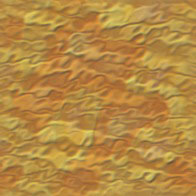
\includegraphics[width=\paperwidth,height=\paperheight]{newton.jpg}}

 
\begin{document}


\begin{frame}{Introduction}
\begin{itemize}
\item 1
\item 2
\item 3
\end{itemize}
\end{frame}


\begin{frame}{Experimental Procedure}
\begin{itemize}
\item 1
\item 2
\item 3
\end{itemize}
\end{frame}


\begin{frame}{Results}
\begin{itemize}
\item 1
\item 2
\item 3
\end{itemize}
\end{frame}



\begin{frame}
\frametitle{Results}
\begin{itemize}
\item 1
\item 2
\item 3
\end{itemize}
\end{frame}


\begin{frame}
\frametitle{Modelling}
\begin{itemize}
\item Conditions
\begin{itemize}
\item part 1
\item part 2
\item part 3
\end{itemize}
\end{itemize}
\end{frame}


\begin{frame}
\frametitle{Discussion}
\begin{itemize}
\item item 1
\item item 2
\item item 3
\end{itemize}
\end{frame}



\begin{frame}{Summary}
\begin{itemize}
\item 1
\item 2
\item 3
\end{itemize}
\end{frame}


\end{document}
